\section{学位论文进展情况}

本章节将概述学位论文的整体进展情况。
首先,将介绍研究的背景,这部分内容将简要阐述量子计算机,模型检测等相关背景。
接着,会详细描述研究的主要内容,包括研究目标、方法论以及预期的贡献。
然后,会探讨在研究过程中遇到的一系列关键问题。
最后,本章节将展示目前已取得的阶段性成果,包括研究内容进展与学术论文撰写进度。

\subsection{研究背景}

模型检测(Model Checking)是一种自动化形式方法,用于验证有限状态系统的性质。模型检测最初由 E. M. Clarke 和 E. A. Emerson 提出\citep{Emerson_1980,Clarke,Clarke_1986},如今已广泛应用于软件和硬件设计。例如,在嵌入式系统中,可以使用 UML 活动图来验证硬件是否符合规范\citep{Grobelna_2015}。

模型检测将待检测的系统建模为一个跃迁系统(transition system),在时序逻辑(temporal logic)中指定待验证的属性。给定模型\(M\) 和属性\(\varphi\),模型检测将验证是否\(M\)满足\(\varphi\)。在不同的模型检测方法中,高级符号模型检查(Advanced Symbolic Model Checking)\citep{Grobelna_2015}使用简化的有序二叉决策图(Reduced Ordered Binary Decision Diagrams,ROBDDs 或 BDDs)\citep{Bryant_1986}来表示状态集合和转移关系。通过迭代调用图像计算算法来计算所有可达状态,判断一个模型是否满足时间属性,直到达到不动点为止。

最近,随着量子计算的发展,关于量子线路的验证技术也在不断发展\citep{viamontes2007checking,burgholzer2020advanced}。其中,利用模型检测方法对线路进行自动化验证也有了一些应用。由于量子线路运算空间随着量子比特的线性增加而指数级膨胀,传统的计算方法并不能很好应对。因此本次研究希望应用基于张量网络(tensor network)的张量决策图(tensor decision diagrams)进行量子模型检测。 

\subsubsection{量子计算简介}

量子计算机(quantum computer)是一种利用量子比特特性进行计算的一种设备。在量子计算中,量子比特的特殊性质允许其同时处于多种状态,这与经典比特的二进制状态不同。量子计算机的状态空间可以用希尔伯特空间(Hilbert space)\(\mathcal{H}\)表示\citep{nielsen2010quantum},即可以进行内积运算(inner product)的复向量空间。比特状态可以用\(\mathcal{H}\)的向量表示,量子门由\(\mathcal{H}\)上的酉算子(unitary operator)表示。

量子线路(quantum circuit)是一种描述量子计算的模型。在量子线路中,通过量子比特的初始化、应用量子门、测量以及其他可能的操作的序列来构建和执行量子计算任务。量子线路通常从左向右阅读,每个量子门的作用是将输入的量子比特状态转变为输出状态,该过程可以认为是量子门的酉矩阵与输入的量子状态的乘积。
\begin{figure}[!htbp]
    \centering
    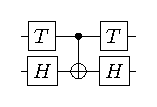
\includegraphics[width=.6\textwidth]{Img/example_cir.pdf}
    \caption{一个量子线路的例子}
    \label{fig:example_cir}
\end{figure}

图\ref{fig:example_cir} 所示的量子线路展示了一个具体的量子线路示例。其中有单比特门\(H=\frac{1}{\sqrt2}\left[\begin{matrix}1&1\\1&-1\\\end{matrix}\right],T=\left[\begin{matrix}1&0\\0&e^{-i\pi/4}\\\end{matrix}\right]\),以及双比特门\(CX=\left[\begin{matrix}\begin{matrix}1&0\\0&1\\\end{matrix}&\begin{matrix}0&0\\0&0\\\end{matrix}\\\begin{matrix}0&0\\0&0\\\end{matrix}&\begin{matrix}0&1\\1&0\\\end{matrix}\\\end{matrix}\right]\)。假设该量子线路的初始状态为\(\left|\psi\right\rangle=\left|\psi_1\right\rangle\left|\psi_2\right\rangle\),则输出状态为\(T\otimes H\cdot CX\cdot T\otimes H\cdot\left|\psi\right\rangle\)。

在量子计算机上可以执行各种算法和计算任务,如量子搜索\citep{Grover_1996}、量子因子分解\citep{shor}和量子模拟\citep{Feynman}等。量子计算的潜力在于其能够在某些特定问题上比经典计算机更高效地进行计算,尤其在处理大规模数据和解决复杂问题方面具有潜在优势。需要对这部分深入了解的读者,可以自行阅读\citep{nielsen2010quantum}。

\subsubsection{跃迁系统}
跃迁系统广泛应用于模型检测中待检测系统的建模,其定义为\citep{baier2008principles}:
\begin{equation}
\mathcal{M}=\{S,Act,\rightarrow,I\}
\end{equation}
其中\(S\)为系统状态集合,\(I\)为系统初态集合,因此满足\(I\subseteq S\)。\(Act\)为系统行为集合。\(\rightarrow\)为系统状态转移关系,即\(\rightarrow\subset S\times Act\times S\)。此外还有\(AP\)为描述系统原子命题。L是标记函数,将状态映射为状态满足的原子命题集合。需要验证的属性\(\varphi\)将表述为命题。


系统的有限路径片段\(\pi\)是一个有限状态序列\(s_0,s_1\ldots s_n\)。\(s_i\)满足\(s_{i-1}\overset{a}{\rightarrow}s_i,a\in Act\),对于所有\(0<i\leq n\),其中\(n\geq 0 \)。无限路径片段\(\pi\)是一个无限状态序列\(s_0,s_1\ldots\),使得对于所有\(i>0\),\(s_{i-1} \overset{a}{\rightarrow}  s_i,a\in Act\)。在路径中\(\pi\left[i\right]=s_i,\pi\left[i\right)=s_i\ldots\)。所有以\(s_0\)为开始的路径,构成了路径集合\(Path\left(s_0\right)\)。

\begin{figure}[!htbp]
    \centering
    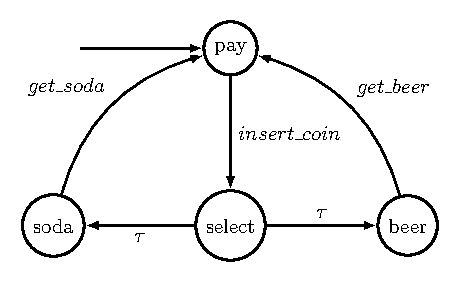
\includegraphics[width=.6\textwidth]{Img/map.pdf}
    \caption{一种简化版的售货机跃迁系统}
    \label{fig:transition-system}
\end{figure}

图\ref{fig:transition-system} 所示的跃迁系统展示了一个简化版的售货机模型。在该模型中,用户投入硬币,进行选择后就可以得到苏打水或者啤酒。在该例子中,系统状态\(S=\{pay,select,soda,beer\}\),系统初态\(I=pay\)。
系统行为\(Act=\{insert\_coin,\tau,get\_soda,get\_beer\}\),其中\(\tau\)表示立即行动符号。转移关系图中已经展示。原子命题可取\(AP=\{paid,drink\}\)。因此\(L\left( pay \right)=\{\varnothing\}\),\(L\left(soda\right)=L\left(beer\right)=\{paid,drink\}\),\(L\left(select\right)=\{paid\}\)。系统的一个路径是\(\pi=pay\ select\ soda\ pay\ selsect\ \ldots\)。此时\(\pi\left[1\right]=slect,\pi\left[1\right)=select\quad soda\quad pay\quad selsect\ldots\)。同时该路径满足\(\pi\in Path\left(pay\right)\)。
量子模型检测的跃迁系统类似。区别在于状态空间用\(\mathcal{H}\),转移关系用酉矩阵。一个量子自动机定义如下:
\begin{align}
    \mathcal{M}=\{\mathcal{H},Act,\{U_\alpha,\alpha\in Act\},\mathcal{H}_0\}
\end{align}
由于目前量子模型检测的发展还比较初期,因此需要验证的属性\(\varphi\)会表示为\(\mathcal{H}\)的一个子空间。
下一节将简要介绍量子模型检测。

\subsubsection{量子模型检测}
随着量子计算硬件规模的快速增长,量子电路的验证成为一个重要问题。开始的研究主要集中在BDD在量子计算下的推广算法,如量子信息决策图(Quantum Information Decision Diagram,或QuIDD)\citep{Viamontes_2003},量子多值决策图(Quantum multiple-valued Decision Diagram,或QMDD)\citep{Seiter_2013}等,从而对组合式量子电路进行等效性检查。显然,随着越来越复杂的物理可实现化的硬件出现,将会出现更加复杂的,更加针对于的,新的验证问题。比如量子存储\citep{Kerckhoff_2010},量子反馈网络\citep{Gough_2008},RUS量子电路\citep{Bocharov_2015}。量子模型检测可以为量子电路的验证提供了更多思路。

量子系统模型检测的早期工作旨在验证量子通信协议\citep{Gay,BALTAZAR_2008,davidson2012model}。后来还有针对分析和验证量子程序的应用\citep{ying2016foundations},比如量子自动机\citep{ying2014model}、量子马尔可夫链\citep{Ying_2013}和超算符值马尔可夫链\citep{feng2013model}的模型检测技术。然而,在这些量子模型检测技术与它们在验证量子电路方面实际应用之间存在巨大差距仍需填补。TDD作为新的数据结构,极大加快了计算过程,有可能深化二者的联系,加快实际应用的出现。

对于量子模型检测的可达性问题的解决,一种直接的解决办法是计算路径上每个状态,然后与待检测属性比较。但是量子计算中状态空间\(\mathcal{H}\)维度\(dim\left(\mathcal{H}\right)=2^n\),其中n为比特数量。即状态空间维数随比特个数指数级增长。

因此需要借助更好的数据结构,更方便的表示量子状态以及量子线路,并计算最终的结果。比如TDD给出了量子电路的紧凑表示,提供了一种方便的实现张量网络各种操作的方式,这些操作对于模拟量子物理系统非常重要。图\ref{fig:P}展示了一个矩阵和TDD形式,其中TDD中的实线表示高边,虚线表示低边。可以明显看到TDD的结构更紧凑。
 	 
\begin{figure}[!htbp]
    \begin{subfigure}[c]{0.4\textwidth}
        \centering
        \includegraphics[width=\textwidth]{Img/matrix_of_tdd.pdf}
        \caption{矩阵$P$的矩阵形式}
        \label{fig:mat_P}
    \end{subfigure}
    \begin{subfigure}[c]{0.4\textwidth}
        \centering
        \includegraphics[height=6cm]{Img/tdd_ex.pdf}
        \caption{矩阵$P$的TDD形式}
        \label{fig:tdd_P}
    \end{subfigure}
    \caption{应用TDD可以减少存储特殊矩阵的资源}
    \label{fig:P}
\end{figure}

TDD特别适用于实现可达性分析和模型检查算法。这是因为基于BDD的模型检查算法中使用的许多优化技术可以推广到收缩量子电路张量网络上\citep{Chaki_2018}。这些为应用TDD解决量子模型检测问题提供了可能的方案。
目前量子模型检测仅仅应用于小规模线路的验证,如何扩展到更大规模电路,是一个难题。

\subsection{研究内容}
在本节中,将探讨本研究的核心内容,即“量子模型检测中的时序逻辑的验证”。
这一研究问题在量子计算领域具有重要的理论与实际意义,关乎量子计算机的精确性和效率。为了解决这一问题,本研究采用了方法论为利用TDD(Tensor Decision Diagram)数据结构来快速模拟量子计算过程。这种方法提高了计算效率,为量子计算提供了更加准确的模拟。

进一步地,研究过程中将探讨四种可能的优化途径,这些途径旨在进一步提升模拟过程的效率。
这四种方法既有来源于经典计算机的思路,也有量子计算机特有的思路。每一种方法都将简要说明。

\subsubsection{时序逻辑的验证}
在量子模型检测中,与经典模型检测一样使用时序逻辑指定待验证的属性\(\varphi\)。时序逻辑命题的运算符有两类\citep{goranko_2023}。状态命题公式(State formulas):\(\varphi ::=a\left|\exists\varphi\right|\forall \varphi\left|\lnot\varphi\right|\varphi\land\psi\),其中\(a\in AP\)。以及路径命题公式(Path formulas):\(\varphi\Colon=O\varphi|\varphi U\psi\)。给定模型的一个状态为\(s\),路径为\(\pi\),则具体满足条件分别如下:
\begin{itemize}
    \item \(s\models a,iff \L\left(s\right)\models a\)
    \item \(s\models\exists\varphi,iff\ \pi\models\varphi\)对一些\(\pi\in Path\left(s\right)\)
    \item \(s\models\forall\varphi,iff\ \pi\models\varphi\)对所有\(π\in Paths\)
    \item \(s\models\lnot\varphi,iff\ s\nvDash\varphi\)
    \item \(s\models\varphi\land\psi,iff\ s\models\varphi\ and\ s\models\psi\)
    \item \(\pi\models O\varphi,iff\ \pi\left[1\right]\models\varphi\)
    \item \(\pi\models\varphi U\psi,iff\ \exists j\geq0\).\(\pi\left[j\right)\models\psi\) 同时对所有\(0\le i<j\)有\(\pi\left[i\right)\models\varphi\)
\end{itemize}


图\ref{fig:path-formula-basic} 展示了两种路径命题公式的直观示意图。


\begin{figure}[!htbp]
    \centering
    \begin{subfigure}[b]{0.8\textwidth}
        \centering
        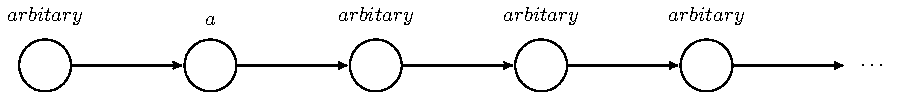
\includegraphics[width=\textwidth]{Img/path_for_Oa.pdf}
    \end{subfigure}
    \\
    \begin{subfigure}{0.8\textwidth}
        \centering
        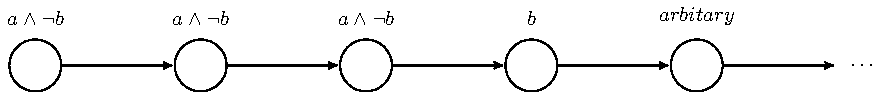
\includegraphics[width=\textwidth]{Img/path_for_aUb.pdf}
    \end{subfigure}
    \caption{$\pi\models O a $与 $\pi\models a U b$的图示}
    \label{fig:path-formula-basic}
\end{figure}
在模型检测中,有三类比较重要的可达性问题,分别是可达性、持续可达性以及重复可达性。过程中主要涉及以下路径命题公式:\(\lozenge\) 表示最终(eventually),\(\square\)表示总是(always),\(\lozenge\square\)表示总是最终(always eventually),\(\square\lozenge\)表示最终总是(eventually always)。其中\(\lozenge\)和\(\square\)具体定义为:
\begin{itemize}
    \item \(\lozenge\varphi\overset{\text{def} }{=} \text{True}U\varphi\)
    \item \(\square\varphi\overset{\text{def} }{=} \neg\lozenge\neg\varphi\)
\end{itemize}
图\ref{fig:path-formula}展示了这两种基本路径命题公式的直观示意图。
\begin{figure}[!htbp]
    \centering
    \begin{subfigure}[b]{0.8\textwidth}
        \centering
        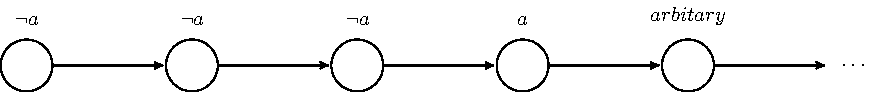
\includegraphics[width=\textwidth]{Img/path_for_Dia.pdf}
    \end{subfigure}
    \\
    \begin{subfigure}{0.8\textwidth}
        \centering
        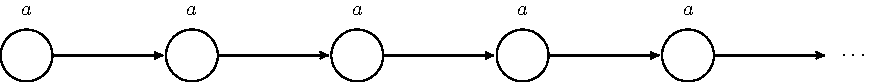
\includegraphics[width=\textwidth]{Img/path_for_SQa.pdf}
    \end{subfigure}
    \caption{$\pi\models\lozenge a$与 $\pi\models\square a$的图示}
    \label{fig:path-formula}
\end{figure}

具体的可满足条件为:
\begin{itemize}
    \item \(\pi\models\lozenge\varphi,iff\exists j\ge0.\pi[j)\models\varphi\)
    \item \(\pi\models\square\varphi,iff\forall j\ge 0.\pi[j)\models\varphi\)
    \item \(\pi\models\lozenge\square\varphi,iff\exists i\ge 0.\forall j\ge i,\pi[j)\models\varphi\)
    \item \(\pi\models\square\lozenge\varphi,iff\forall i\ge 0.\exists j\ge i,\pi[j)\models\varphi\)
\end{itemize}
基于此三种可达性问题定义分别如下:
\begin{itemize}
    \item 可达性:\( Pr^{\mathcal{M}}(s \models \lozenge G) = Pr^M(\pi \models \lozenge G : \pi \in \text{Paths}(s))\)
    \item 持续可达性:\( Pr^{\mathcal{M}}(s \models \lozenge \square G) = Pr^M(\pi \models \lozenge \square G : \pi \in \text{Paths}(s))\)
    \item 重复可达性:\( Pr^{\mathcal{M}}(s \models\square \lozenge G) = Pr^M(\pi \models \square\lozenge G : \pi \in \text{Paths}(s))\)
\end{itemize}

\subsubsection{研究方法}
本次研究的主要目的是借助TDD数据结构,构建能快速计算量子模型检测中可达问题的方案。因此主要采用的方法是模拟量子计算。本次研究的主要挑战在于尽可能减少程序的运行时间。为此,需要采用一系列方法来开发更有效的算法,以优化TDD操作和收缩张量网络。其中包括开发新技术来分割张量网络和优化TDD结构。
下面简单介绍以下具体研究方法。

\begin{myen}

\item \label{addition}关于常用的量子线路划分方法,
第一种被称为addition\citep{chen2018classical}。将量子电路视为张量网络,首先将一个量子电路C转换成无向图G。G中的每个节点表示量子电路的一个索引,并且如果它们是相同门的输入或输出索引,则在G中连接两个节点。并且当满足以下两个条件之一时输入和输出索引不变:
\begin{itemize}
	\item 是对角线量子门的输入和输出索引;
	\item 是受控门的控制比特位的输入和输出索引。
\end{itemize}
	
图\ref{fig:addition}展示了Grover\_3电路图的索引链接图。该图描述了量子电路的连通性,通过选择图中连通度最大的索引可以对电路进行分割。因此选择图中连通度较大的$x_1^1,x_1^3x_2^1$可以对电路进行较好的划分。
 
\begin{figure}[!htbp]
	\centering
	\includegraphics[height=5cm]{Img/cir_index_graph.pdf}
	\caption{Grover\_3的索引连接图}
	\label{fig:addition}
\end{figure} 

\item 另一种常用的电路划分方法成为contraction。在这一方法中,将量子电路划分为若干个较小的部分,其收缩等于原始电路。对于两个预设整数参数k1和k2,将电路划分为若干小电路。其中每个小电路涉及最多k1个量子比特,并且与至多跨越不同部件的k2个多比特门相连。图\ref{fig:contraction}展示了对Bit flip电路进行k1=3,k2=2的拆分结果。
\begin{figure}[!htbp]
	\centering
	\includegraphics[height=4.5cm]{Img/cir_contraction.pdf}
	\caption{对Bit flip电路进行contraction的拆分}
	\label{fig:contraction}
\end{figure} 


\item \label{contraction}在BDD中,索引的顺序很重要。因为索引顺序会直接影响BDD的大小。一个良好的变量顺序可以使得BDD比一个糟糕的变量顺序小得多。图\ref{fig:bdd-compare}的了两张图都表示了布尔函数ƒ(x1,...,x8)=x1x2+x3x4+x5x6+x7x8,但图\ref{fig:bdd-good}的结构更简单。其中图\ref{fig:bdd-bad}的索引顺序为\{x1,x3,x5,x7,x2,x4,x6,x8\},图\ref{fig:bdd-good}的索引顺序为\{x1,x2,x3,x4,x5,x6,x7,x8\}。找到一个好的索引顺序是一个NP问题。在工程实现中,目前只能通过小规模电路上寻求规律,然后在更大规模电路中应用较优顺序。

\begin{figure}[!htbp]
	\centering
	\begin{subfigure}[b]{.4\textwidth}
        \centering
        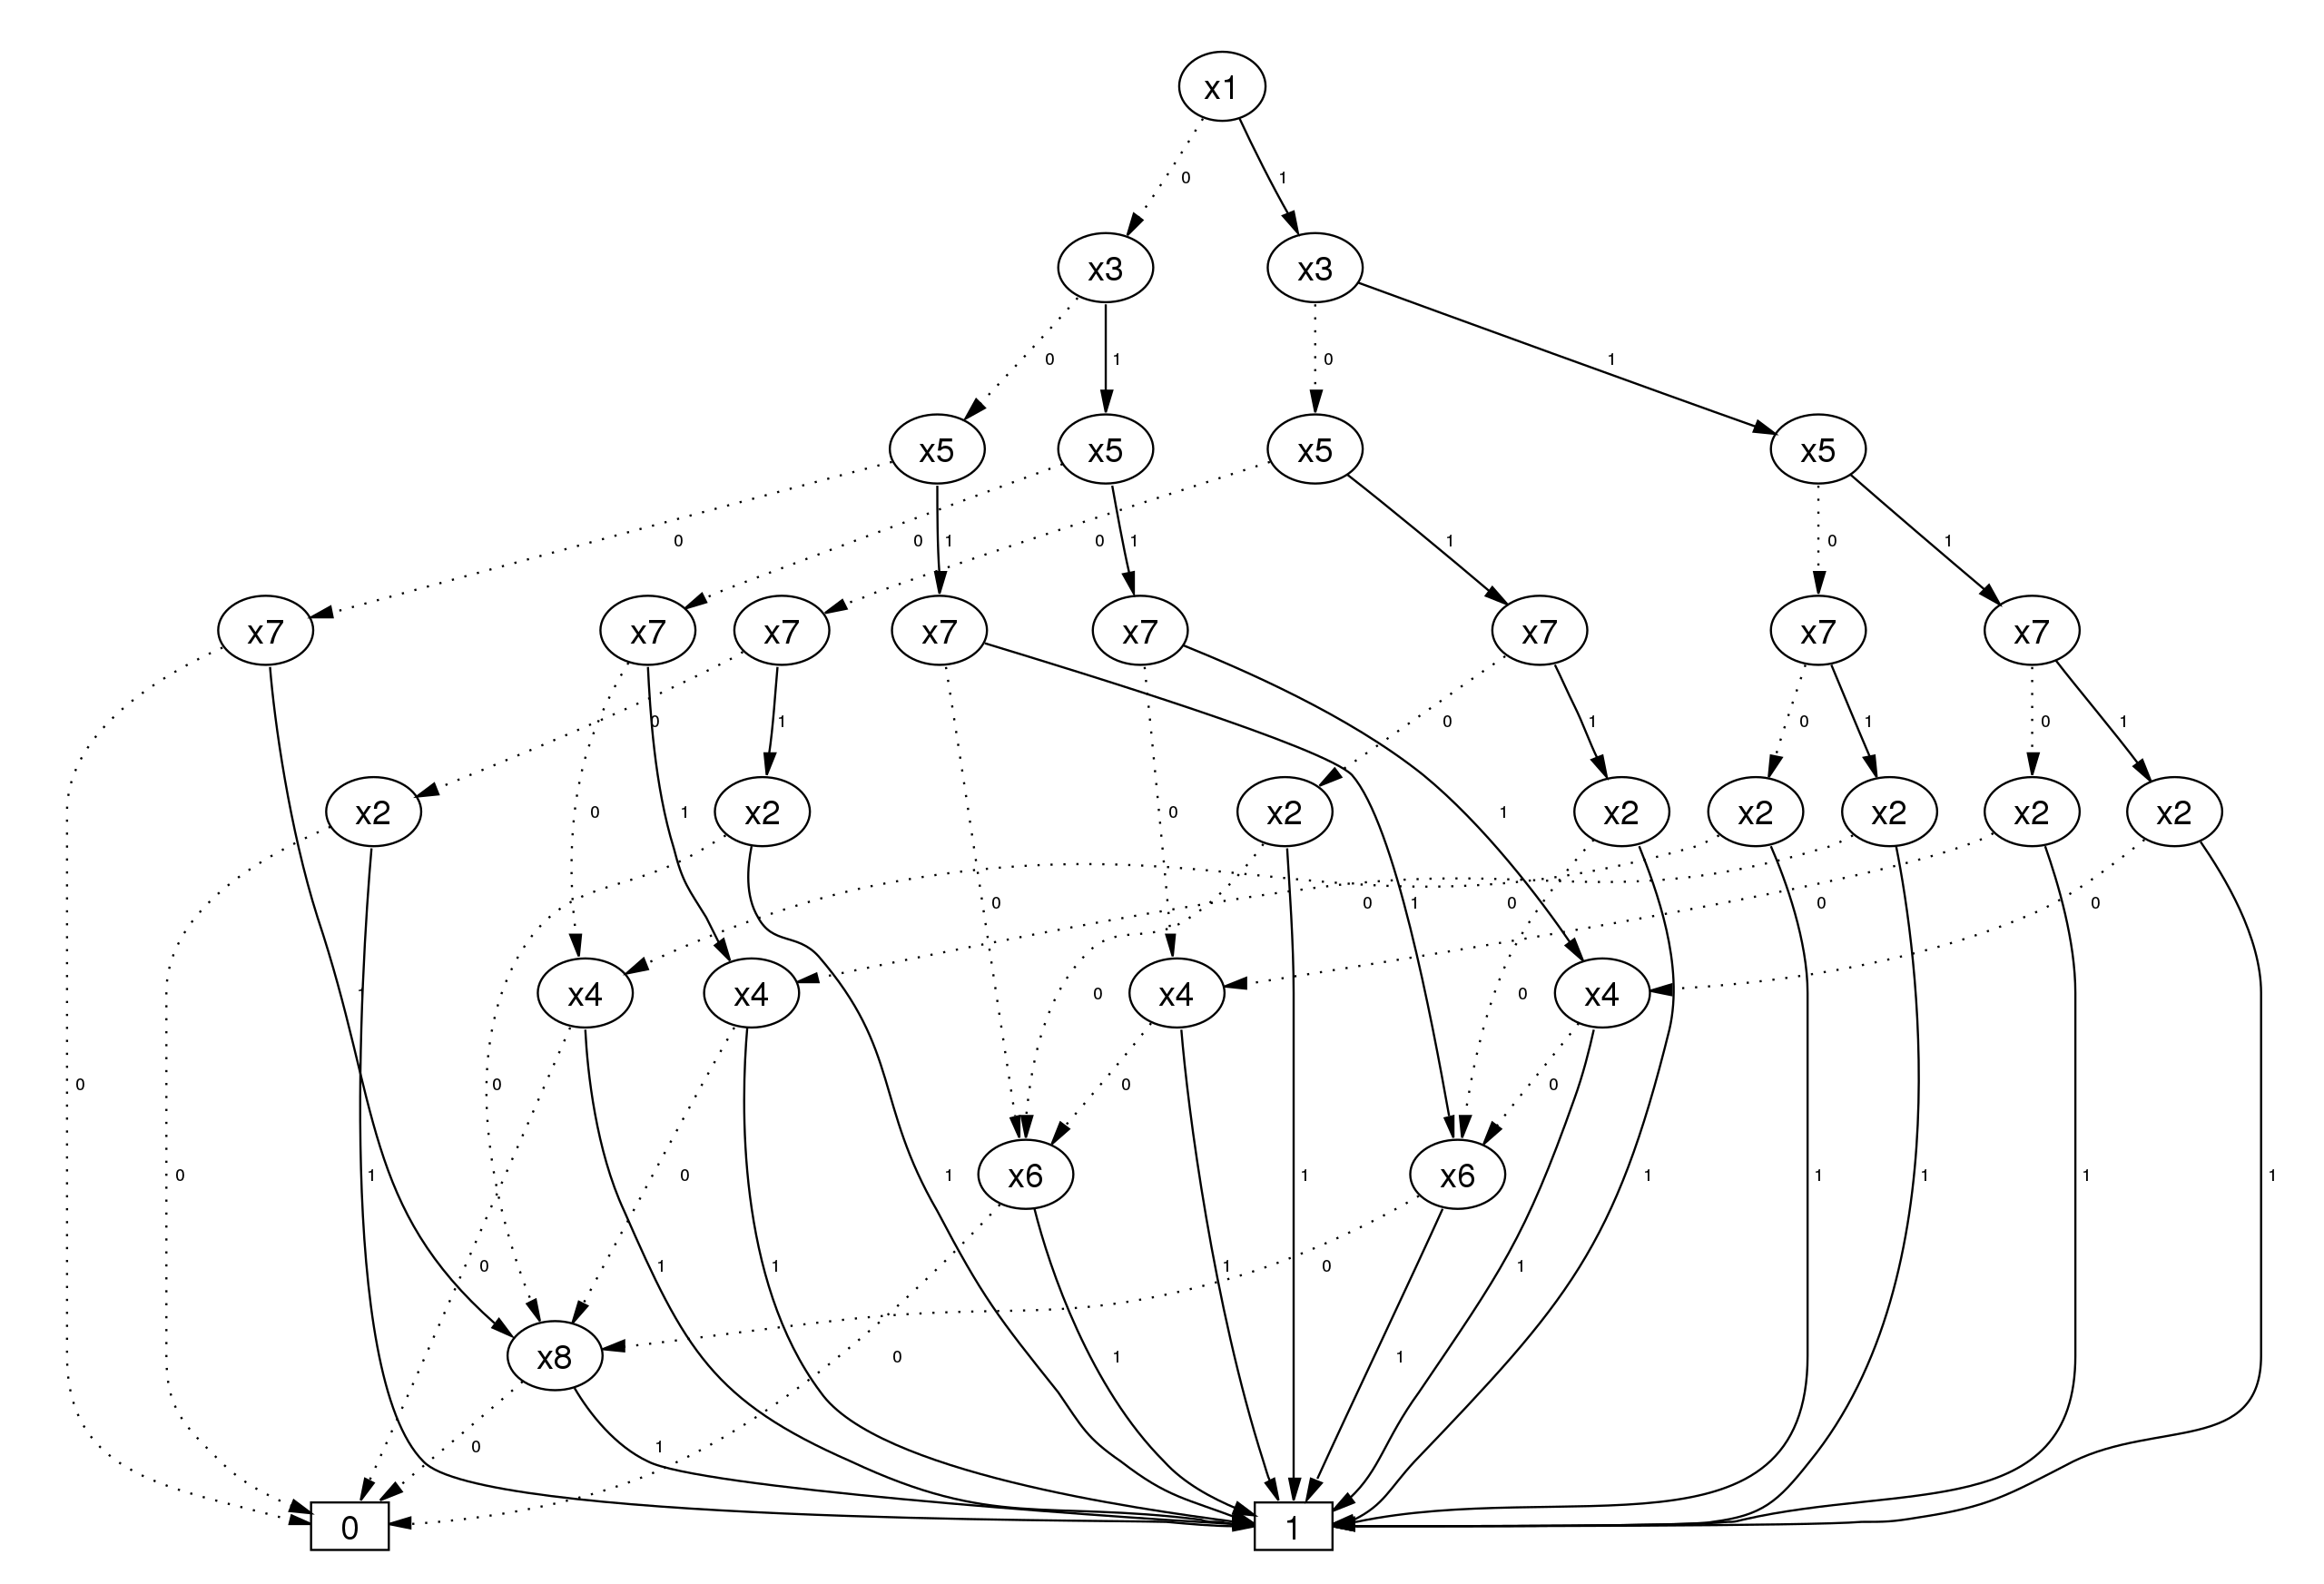
\includegraphics[height=4.5cm]{Img/BDD_Variable_Ordering_Bad.svg.pdf}
		\caption{索引顺序为\{x1,x3,x5,x7,x2,x4,x6,x8\}}
		\label{fig:bdd-bad}
	\end{subfigure}
	\begin{subfigure}[b]{.4\textwidth}
        \centering
        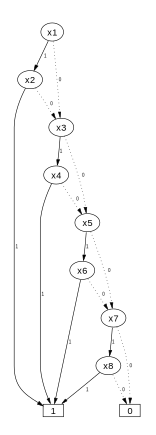
\includegraphics[height=5cm]{Img/BDD_Variable_Ordering_Good.svg.pdf}
		\caption{索引顺序为\{x1,x2,x3,x4,x5,x6,x7,x8\}}
		\label{fig:bdd-good}
	\end{subfigure}
	\caption{同一布尔函数在不同索引顺序下的结构图\citep{wiki:bdd}}
	\label{fig:bdd-compare}
\end{figure}


\item 由于量子状态都在同一希尔伯特空间中。因此作用某些算子后,不同的量子状态可能等价。
当存储算子的资源少于存储状态的资源时,就有可能存储算子表示不同的状态\citep{vinkhuijzen2023limdd}。图\ref{fig:qmdd-example}表示了一个QMDD的例子,应用等价性,可以化简为图\ref{fig:limdd-example}。
TDD也可以应用类似技术,进行进一步化简,从而降低资源要求。
\begin{figure}[!htbp]
    \centering
    \begin{subfigure}[b]{.4\textwidth}
        \centering
        \includegraphics[height=6cm]{Img/limdd.pdf}
        \caption{一个QMDD示例}
        \label{fig:qmdd-example}
    \end{subfigure}
    \begin{subfigure}[b]{.4\textwidth}
        \centering
        \includegraphics[height=6cm]{Img/limdd_reduce.pdf}
        \caption{应用等价性化简图\ref{fig:qmdd-example}}
        \label{fig:limdd-example}
    \end{subfigure}
\end{figure}
\end{myen}
\subsection{存在的问题}
在本研究过程中,主要遇到了两个问题,这些问题对研究的深入发展和实际应用产生了重要影响。

首先,面临的一个关键挑战是如何将所提出的方法扩展应用到更大规模的实例。这不仅涉及到算法的效率问题,还包括数据处理能力的提升。对于实现验证量子计算算法在更广泛领域的应用至关重要。为了解决这一挑战,目前采用电路拆分方法来降低TDD的资源消耗,并挖掘可能的并行计算机会。此外,还计划应用更灵活的索引策略和limdd的思路,以期达到更高效的处理效果。

其次,另一个重要的问题是如何将研究方法应用于更加实用的示例。这是将理论研究转化为实际应用的关键一步。目前考虑的主要方向是将此方法应用到量子线路设计,即QDA(Quantum Design Automation)领域。
计划未来能够将本研究成果应用于不同的synthesis算法的验证等价性中,从而在量子计算的实际应用中发挥更大的作用。


\subsection{阶段性成果}
\subsubsection{研究内容进展}
在模型检测中,image computation指的是在给定当前状态$s_i\in S$和行为$\alpha\in Act$的情况下计算接下来的状态。
目前,关于使用TDD对量子的image computation的计算已经完成。表\ref{table:time}给出了在不同电路拆分技术下Grover算法的计算时间,单位为秒。其中basic表示没有使用优化技术,addition表示使用研究方法\ref{addition}的addition优化技术,contraction表示使用研究方法\ref{contraction}中的contraction优化技术。“-”表示超过一小时的运行上限。
\begin{table}[!htbp]
    \centering
    \begin{tabular}{llllllllll}
        \hline
        \multirow{2}{*}{Benchmark} &  & \multicolumn{2}{c}{basic} &  & \multicolumn{2}{c}{addition} &  & \multicolumn{2}{c}{contraction} \\ \cline{3-4} \cline{6-7} \cline{9-10} 
                                   &  & time        & max \#node       &  & time          & max \#node        &  & time           & max \#node          \\ \hline
        Grover\_15 &   & 19.33  & 15785     &   & 17.35      & 15099  & & 1.61 & 597  \\
        Grover\_18 &   & 76.47  & 61694     &   & 66.02      & 60332  & & 2.41 & 516  \\
        Grover\_20 &   & 294.65 & 243946    &   & 259.87     & 241240 & & 4.39  & 1036 \\ 
        Grover\_40 &   & -      &           &   & -          &        & & 2953.57 & 851973 \\
        \hline
        QFT\_15     &  & 34.64   & 65536   &  & 18.88  & 32770   &  & 0.08 & 63  \\
        QFT\_18     &  & 282.12  & 524288  &  & 148.13 & 262146 &   & 0.10  & 31  \\
        QFT\_20     &  & 1199.21 & 2097152 &  & 655.19 & 1048578 &  & 0.12 & 63  \\
        QFT\_30     &  & -       &         &  & -      &        &  & 0.29 & 31  \\
        QFT\_50     &  & -       &         &  & -      &        &  & 1.02 & 51  \\
        QFT\_100    &  & -       &         &  & -      &        &  & 7.14 & 101 \\
        \hline
        BV\_100     &  & 7.36    & 596     &  & 7.43      & 596     &  & 0.41           & 102 \\
        BV\_200     &  & 31.57   & 1196    &  & 30.03     & 1196    &  & 1.70           & 202 \\
        BV\_300     &  & 75.66   & 1796    &  & 75.56     & 1796    &  & 4.28           & 302 \\
        BV\_400     &  & 146.47  & 2396    &  & 145.40    & 2396    &  & 9.18           & 402 \\
        BV\_500     &  & 244.15  & 2996    &  & 223.90    & 2996    &  & 16.31          & 502 \\
        \hline
        GHZ\_100    &  & 0.38    & 595     &  & 0.13      & 301    &  & 0.18           & 200 \\%& 0.03    
        GHZ\_200    &  & 0.72    & 1195    &  & 0.37      & 601    &  & 0.48           & 400 \\%& 0.12     
        GHZ\_300    &  & 1.29    & 1795    &  & 0.62      & 901    &  & 0.80           & 600 \\%& 0.24     
        GHZ\_400    &  & 2.03    & 2395    &  & 1.00      & 1201    &  & 1.26           & 800 \\%& 0.42     
        GHZ\_500    &  & 2.96    & 2995    &  & 1.45      & 1501    &  & 1.72           & 1000\\%& 0.62     
        \hline
        QRW\_15     &  & 36.86   & 13122     &  & 24.59     & 10882     & & 7.16  & 222 \\
        QRW\_18     &  & 139.76  & 90538     &  & 84.69     & 37064     & & 11.23 & 226 \\
        QRW\_20     &  & 341.05  & 265614    &  & 218.29    & 107714    & & 14.31 & 404 \\
        QRW\_30     &   &-       &          &  &-          &          & & 36.82 & 404 \\
        QRW\_50     &   &-       &          &  &-          &          & & 118.08 & 404 \\
        QRW\_100    &   &-       &          &  &-          &          & & 692.08 & 436 \\
        \hline
    \end{tabular}
    \caption{对不同测试实验应用image computation}
    \label{table:time}
\end{table}

通过对比不同优化技术下的计算时间,可以看到使用优化技术能够显著降低计算时间。例如,在Grover-20的例子中,使用"contraction"优化技术的情况下,计算时间从294秒降低到了4秒。这表明优化技术在提高计算效率方面起到了积极的作用。同时,表\ref{table:addition}展示了对同一线路,即Grover\_15应用不同的addition参数的时间,可以看到合适的参数
选择也是非常重要的。
\begin{table}[!htbp]
    \centering
    \begin{tabular}{c|ccccccccccccccc}
        \rowcolor[HTML]{FFFFFF} 
        \diagbox{k1}{k2}                         & 1                           & 2                           & 3                           & 4                           & 5                           & 6                           & 7                          & 8                           & 9                           & 10                          & 11                          & 12                          & 13                          & 14                          & 15                          \\\hline
            \rowcolor[HTML]{FFFFFF} 
    1                          & 2.8                                              & 2.2                         & 2.1                         & \cellcolor[HTML]{CCC0DA}2.0 & \cellcolor[HTML]{CCC0DA}1.9 & \cellcolor[HTML]{CCC0DA}2.0                      & 2.1                        & \cellcolor[HTML]{CCC0DA}2.0 & 2.1                         & \cellcolor[HTML]{CCC0DA}2.0 & \cellcolor[HTML]{CCC0DA}2.0 & 2.1                         & 2.2                         & 2.1                         & 2.1                         \\ \cline{3-7}
    \rowcolor[HTML]{CCC0DA} 
    
    \rowcolor[HTML]{FFFFFF} 
    3                          & \multicolumn{1}{l|}{\cellcolor[HTML]{FFFFFF}2.2} & \cellcolor[HTML]{CCC0DA}1.9 & \cellcolor[HTML]{CCC0DA}1.8 & \cellcolor[HTML]{CCC0DA}1.6 & \cellcolor[HTML]{CCC0DA}2.0 & \multicolumn{1}{l|}{\cellcolor[HTML]{CCC0DA}1.9} & 2.1                        & 2.1                         & 2.5                         & 2.3                         & 2.7                         & 2.3                         & 3.1                         & 2.8                         & 3.3                         \\
    \rowcolor[HTML]{FFFFFF} 
    4                          & \multicolumn{1}{l|}{\cellcolor[HTML]{FFFFFF}2.3} & \cellcolor[HTML]{CCC0DA}1.8 & \cellcolor[HTML]{CCC0DA}2.0 & \cellcolor[HTML]{CCC0DA}1.7 & \cellcolor[HTML]{CCC0DA}2.0 & \multicolumn{1}{l|}{\cellcolor[HTML]{FFFFFF}2.1} & 2.2                        & 2.1                         & 2.6                         & 2.3                         & 2.8                         & 2.7                         & 3.3                         & 3.0                         & 3.3                         \\
    \rowcolor[HTML]{FFFFFF} 
    5                          & \multicolumn{1}{l|}{\cellcolor[HTML]{FFFFFF}2.2} & \cellcolor[HTML]{CCC0DA}1.7 & \cellcolor[HTML]{CCC0DA}1.9 & \cellcolor[HTML]{CCC0DA}1.6 & \cellcolor[HTML]{CCC0DA}1.9 & \multicolumn{1}{l|}{\cellcolor[HTML]{CCC0DA}2.0} & 2.3                        & \cellcolor[HTML]{CCC0DA}1.9 & 2.5                         & 2.3                         & 2.8                         & 2.7                         & 3.4                         & 3.0                         & 3.6                         \\
    \rowcolor[HTML]{FFFFFF} 
    6                          & \multicolumn{1}{l|}{\cellcolor[HTML]{FFFFFF}2.1} & \cellcolor[HTML]{B1A0C7}1.5 & \cellcolor[HTML]{CCC0DA}1.8 & \cellcolor[HTML]{CCC0DA}1.7 & 2.2                         & \multicolumn{1}{l|}{\cellcolor[HTML]{CCC0DA}1.9} & 2.5                        & 2.2                         & 2.9                         & 2.8                         & 3.1                         & 2.9                         & 3.7                         & 3.7                         & 4.2                         \\
    \rowcolor[HTML]{FFFFFF} 
    7                          & \multicolumn{1}{l|}{\cellcolor[HTML]{FFFFFF}2.1} & \cellcolor[HTML]{CCC0DA}1.5 & \cellcolor[HTML]{CCC0DA}1.9 & \cellcolor[HTML]{CCC0DA}1.6 & 2.2                         & \multicolumn{1}{l|}{\cellcolor[HTML]{CCC0DA}1.9} & 2.5                        & 2.2                         & 2.8                         & 3.0                         & 3.6                         & 3.3                       & 4.2                         & 5.7                         & 5.0                         \\
    \rowcolor[HTML]{FFFFFF} 
    8                          & \multicolumn{1}{l|}{\cellcolor[HTML]{CCC0DA}2.0} & \cellcolor[HTML]{CCC0DA}1.7 & \cellcolor[HTML]{CCC0DA}1.8 & \cellcolor[HTML]{CCC0DA}1.7 & 2.1                         & \multicolumn{1}{l|}{\cellcolor[HTML]{CCC0DA}2.0} & 2.4                        & 2.2                         & 2.8                         & 2.8                         & 3.7                         & 3.4                         & 4.3                         & 4.8                         & 5.2                         \\
    \rowcolor[HTML]{FFFFFF} 
    9                          & \multicolumn{1}{l|}{\cellcolor[HTML]{FFFFFF}2.1} & \cellcolor[HTML]{B1A0C7}1.5 & \cellcolor[HTML]{CCC0DA}2.0 & \cellcolor[HTML]{B1A0C7}1.4 & 2.2                         & \multicolumn{1}{l|}{\cellcolor[HTML]{CCC0DA}2.0} & 2.5                        & \cellcolor[HTML]{CCC0DA}2.0 & 3.3                         & 2.9                         & 3.7                         & 3.5                         & 4.9                         & 4.7                         & 5.8                         \\ \cline{3-7}
    \rowcolor[HTML]{FFFFFF} 
    10                         & 2.3                                              & \cellcolor[HTML]{CCC0DA}1.9 & 2.3                         & \cellcolor[HTML]{CCC0DA}1.6 & 2.6                         & 2.7                                              & 3.1                        & 2.2                         & 4.0                         & 3.6                         & 4.6                         & 3.9                         & 5.6                         & 5.2                         & 7.5                         \\
    \rowcolor[HTML]{FFFFFF} 
    11                         & 3.2                                              & 3.2                         & 3.5                         & 3.1                         & 4.7                         & 4.2                                              & 5.6                        & 4.2                         & 6.8                         & 7.2                         & 7.6                         & 6.3                         & 9.0                         & 8.1                         & \cellcolor[HTML]{8DB4E2}11  \\
    \rowcolor[HTML]{FFFFFF} 
    12                         & 5.6                                              & 6.0                         & 7.2                         & 6.0                         & 8.3                         & 9.0                                              & 8.9                        & 7.8                         & \cellcolor[HTML]{8DB4E2}11  & \cellcolor[HTML]{8DB4E2}11  & \cellcolor[HTML]{8DB4E2}12  & \cellcolor[HTML]{8DB4E2}11  & \cellcolor[HTML]{8DB4E2}12  & \cellcolor[HTML]{8DB4E2}15  & \cellcolor[HTML]{8DB4E2}16  \\
    \rowcolor[HTML]{8DB4E2} 
    \cellcolor[HTML]{FFFFFF}13 & 11                                               & 12                          & 14                          & 12                          & 15                          & 18                                               & 18                         & 15                          & 18                          & 20                          & 18                          & 32                          & 32                          & 30                          & 25                          \\
    \rowcolor[HTML]{8DB4E2} 
    \cellcolor[HTML]{FFFFFF}14 & 20                                               & 21                          & 24                          & 32                          & 31                          & 44                                               & 77                         & 50                          & 86                          & \cellcolor[HTML]{538DD5}109 & 68                          & \cellcolor[HTML]{538DD5}133 & 70                          & \cellcolor[HTML]{538DD5}119 & \cellcolor[HTML]{538DD5}142 \\
    \rowcolor[HTML]{538DD5} 
    \cellcolor[HTML]{FFFFFF}15 & \cellcolor[HTML]{8DB4E2}28                       & \cellcolor[HTML]{8DB4E2}30  & \cellcolor[HTML]{8DB4E2}31  & \cellcolor[HTML]{8DB4E2}53  & \cellcolor[HTML]{8DB4E2}69  & 111                                              & \cellcolor[HTML]{8DB4E2}85 & \cellcolor[HTML]{8DB4E2}81  & 102                         & 153                         & 114                         & 130                         & 166                         & 162                         & 235                        
                     
    \end{tabular}
    \caption{对grover\_15应用不同的addition 参数}%calculating the 
    \label{table:addition}
\end{table}
  
在技术实现上,构建了两个版本的量子线路转化为TDD的工具,分别基于C语言和Python语言。这些工具的开发对于实现我们的研究方法至关重要,提高了实验的灵活性和效率。

\subsubsection{学术论文进展:}
在学术论文撰写方面的进展包括:
\begin{itemize}
    \item 完成了学术论文中关于研究背景的详细调查和综述,这部分内容主要包括了量子模型检测的背景知识与重要性。
    \item 撰写了研究内容的方法论部分,详细描述了主要的研究方法和实验设计。阐述了我们的研究方法,并详细介绍了方法的实施步骤和预期目标。
\end{itemize}
